%************************************************
\chapter[Caching of Reaction networks]{Caching and Exploration of Reaction Networks}
\label{ch:cache_in_crns} %
%************************************************

{\sffamily\slshape The text in this chapter is identical to Section 2.5, Section 4 and Appendix A of the preprint at \href{https://arxiv.org/abs/2504.10609}{arXiv.2607.04160}.\\}

Stochastic simulations in reaction networks naturally exhibit temporal locality in the reactions they explore. At any given stage of the simulation, the system state is typically dominated by a small subset of molecular classes with high counts, while the rest of the molecular classes have a low abundance. As a result, collisions repeatedly involve the same molecular pairs, and the same reaction templates are applied to these pairs across many consecutive simulation steps. This effect is particularly pronounced during early and intermediate phases of the simulation, where a limited set of precursor molecules drives most of the reactivity, as well as in regimes where the system approaches steady state. Consequently, the expensive operation of enumerating reaction instances for a given molecular pair and reaction template is often redundantly repeated, even though the underlying graph-theoretic computation yields identical results each time. Exploiting this temporal locality through caching allows the simulation to reuse previously computed reaction instances, thereby accelerating exploration of large reaction networks using the algorithm described in Chapter~\ref{ch:stoc_explore} without altering the stochastic trajectory of the system.

\section{Caching Scheme}
\label{cacheScheme}

In more detail, the framework employs a caching strategy in which reaction instances generated by applying a template $r$ to a molecular pair $(m_1, m_2)$ are cached in a dictionary keyed by the ordered tuple $(m_1, m_2, r)$. Subsequent requests involving the same pair and template are served directly from the cache, bypassing recomputation.  This avoids repeated subgraph isomorphism checks between the left-hand side of the reaction template and the union of the molecular graphs $m_1 \cup m_2$, as well as the subsequent enumeration of product graphs resulting from valid instantiations of the template. 
Since subgraph matching and transformation of the union of the molecular graphs $m_1 \cup m_2$ to the product graphs are among the most computationally expensive operations in rule-based chemical simulations, \emph{memoizing} their outcomes can significantly accelerate the simulation, particularly in large systems where these operations are invoked frequently. This form of memoization is conceptually distinct from earlier caching approaches used in kinetic Monte Carlo simulations, which typically store interaction energies between particles and lattice sites~\cite{kmc_cache}. In contrast, the present framework caches reaction structure, enabling acceleration of stochastic simulations in generative, graph-based chemical spaces.

A \emph{cache hit} occurs when the reaction instances for a requested molecular pair and template are found in memory; otherwise, the request results in a \emph{cache miss} and the reaction instances are recomputed. Cache lookups are substantially faster than recomputation, provided that the cache data structures are designed to support efficient indexing and retrieval. The specific data structure and retrieval policy used in the cache are described in Section~\ref{crp}.

As we demonstrate empirically in Section~\ref{cache_effects}, reuse of cached reaction instances does enable measurable speed-ups in the simulation.
However, increasing the cache size does not proportionally improve performance. The speed-up becomes increasingly marginal as the cache size is increased: larger caches incur higher lookup and management costs, which can partially offset the gains from avoiding recomputation.
Moreover, once the cache reaches its maximum capacity, newly generated reaction instance blocks must overwrite existing entries. In this work, a least-recently-used (LRU) replacement policy is employed, in which the reaction instance block that has not been accessed for the longest time is replaced. More sophisticated policies could incorporate access frequency or attempt to predict future reuse. Ideally, reaction instances that are unlikely to be requested again would be evicted preferentially, but such foresight is difficult to achieve in a stochastic and evolving chemical system.

An additional positive consequence of using a caching scheme is that it stores a partial view of the reaction network explored during the simulation. Although the simulation algorithm in Algorithm~\ref{generate_network} does not require explicit construction or storage of the full underlying network, the cache implicitly retains a subnetwork consisting of frequently sampled reaction instances. By varying the cache size and replacement policy, different regions of the explored reaction network can be preferentially retained, without altering the stochastic trajectory of the simulation itself. This decoupling of network storage from system dynamics provides a mechanism for selectively recording and analysing portions of large reaction networks while preserving the generative nature of the simulation.

\section{Cache Replacement Policy}
\label{crp}

The cache streams in reaction instances until it is full, and thereafter overwrites existing reaction instances with incoming ones according to a cache replacement policy. The optimal cache replacement algorithm OPT~\cite{cache_opt} would overwrite the reaction instances that will not be requested for the largest number of simulation steps in the future. However, it is difficult to predict after how many steps a reaction would be requested again, in particular in a stochastic simulation.

\begin{figure}[!bh]
    \centering
    \begin{subfigure}{0.30\textwidth}
        \centering
        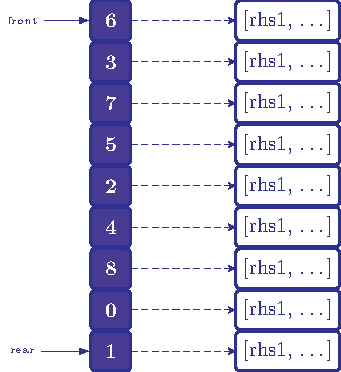
\includegraphics[scale=0.5]{graphics/chapter7/cache.pdf}
        \caption{Depiction of the ordered dictionary used as the cache data structure.}
        \label{fig:cache}
    \end{subfigure}% 
    \hfill
    \begin{subfigure}{0.32\textwidth}
        \centering
        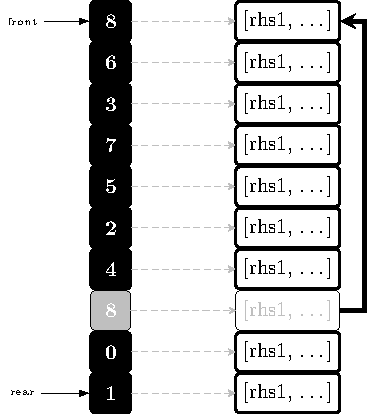
\includegraphics[scale=0.5]{graphics/chapter7/cache_hit.pdf}
        \caption{Cache state after a cache hit moves the requested element to the front.}
        \label{fig:cache_hit}
    \end{subfigure}% 
    \hfill
    \begin{subfigure}{0.32\textwidth}
        \centering
        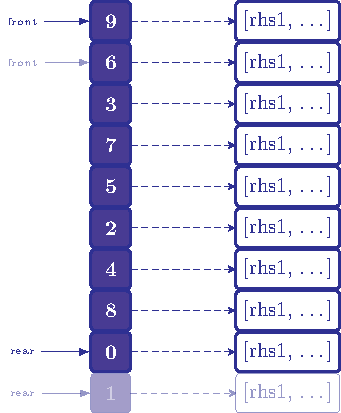
\includegraphics[scale=0.5]{graphics/chapter7/cache_miss.pdf}
        \caption{Cache state after a cache miss removes the rear element and inserts the new element at the front.}
        \label{fig:cache_miss}
    \end{subfigure}
    \caption{The LRU caching policy implemented via an ordered dictionary. A key in the dictionary is formed by a canonical representation of two molecular graphs $(m_1,m_2)$ and the index of the reaction template $r$, while each value is a list containing the right hand sides of the reaction instances computed by applying all matches found between the left hand side of $r$ and the union of the molecular graphs $m_1\cup m_2$. For brevity, the keys are represented by single digit numbers, and the values by abstracted lists. Note that a value might be null for some keys, if the left hand side of $r$ does not match $m_1\cup m_2$. A cache hit results in reordering the entries in the dictionary, by moving the matched query to the front of the dictionary as shown in Figure~\ref{fig:cache_hit}. On a cache miss, the least recently used element (which is the element at the rear of the dictionary) is removed and the new element is added to the front of the dictionary as shown in Figure~\ref{fig:cache_miss}.}
    \label{fig:cache_model}
\end{figure}

Two simple cache replacement policies without significant overhead costs of tracking the access history of cache elements are random replacement and first-in first-out queue. These require minimal bookkeeping but often result in poor hit rates. The cache replacement policy used in this work is that the \emph{least recently used} (LRU) entry is overwritten. This policy assumes that reaction instances that were more recently used in the past would be requested closer in the future. We maintain what in Python is called an \emph{ordered dictionary}~\cite{ordered_dict_py} (essentially a linked list whose elements can be accessed via a hash function) containing the already computed reaction instance groups. In the (key,value)-pairs of the dictionary, a key is composed of a molecule pair $(m_1,m_2)$ and a reaction template $r$, and the value is a list of all the reactions possible to generate by applying $r$ to $(m_1,m_2)$. The most recently used cache element is the first entry of the ordered dictionary, while the least recently used element is the last, as shown in Figure~\ref{fig:cache}. Note that the choice of keys fits the working of Algorithm~\ref{generate_network}, which during the generation of a candidate transition for a state exactly has the colliding pair of molecules and the selected reaction template available (whereas it has no knowledge of their time of last use). On a cache hit, the requested cache element is retrieved from the ordered dictionary and moved to the front of the ordered dictionary, since it now is the most recently used cache element. This is shown in Figure~\ref{fig:cache_hit}. On a cache miss, the least recently used element, which is at the end of the dictionary, is removed. The new element is pushed to the front of the ordered dictionary, as shown in Figure~\ref{fig:cache_miss}. This ensures that the elements in the dictionary are ordered by the the number of steps lapsed since they were requested last. Operations of an ordered dictionary have expected $\mathcal{O}(1)$ runtime (as follows from the runtimes of the underlying hash table and linked list), hence the cache operations have that same runtime.

This algorithm can be shown to result in at most $N$ times more cache misses than OPT (where $N$ is the size of the cache)~\cite{lru_cache_performance}. The worst case occurs when $N+1$ queries are accessed sequentially in an iterative manner. The $(N+1)$th data element overwrites the first element which was the least recently used element. This pattern continues in all subsequent iterations, which therefore all will result in cache misses. These cyclic access patterns, though rare, might occur during the stochastic simulation. In those cases the cache replacement policy might be improved by overwriting the cache element whose $k$-th last request was furthest in the past. Another alternative is to keep track of the frequency of requests of each cache element and overwrite the least \emph{frequently} requested element on a cache miss. However, keeping a count of the request frequency of each cache element would require a third data structure for the necessary bookkeeping, which is not as straight-forward as ordering the cache elements in the linked list by their recency of requests. 
Also, older cache elements would tend to have more requests than recent ones, leading to the more recent cache elements being overwritten. A frequency based caching policy would retain such non-recent cache elements with higher frequency of access in contract to a recency of use based policy.

\section{Effects of Caching}
\label{cache_effects}

To identify a cache size that optimizes performance, we on the pre-biotic formose system studied in Section~\ref{exp} performed $100$ independent simulation runs for each candidate cache size $2^i$, $i = 0, 1, 2,\dots, 20$. For each run, we recorded the wall-clock time required to execute $10^6$ simulation steps and the average cache hit rate (the fraction of requests resulting in a cache hit). Unless otherwise stated, flows are not enabled. The results are summarized in Figure~\ref{fig:cacheSizeEffects}.

As expected, increasing the cache size leads to a higher cache hit rate (blue markers). The improvement is initially rapid and reaches an inflection point at cache size of $2^8$, beyond which the improvement slows down. There is still improvement up to a cache capacity of $2^{15} = 32768$ (with the corresponding cache hit rate being $0.977\pm0.03$), after which the hit rate settles at just below the maximum possible value of one.
A similar saturation effect is observed in the simulation runtime: enlarging the cache leads to substantial speedups up from $305\pm 3$ seconds to $148\pm 3$ seconds, with an inflection point at size $2^{8}$ and no substantial improvements after size $2^{15}$.
The lack of improvement after increasing the cache size beyond $2^{15}$ probably suggests that the number of active cache keys in the system is around~$2^{15}$. On increasing the cache size beyond this, one cannot expect further improvements, and the runtime flattens out to a value dominated by the execution of the rest of the actions during the simulation. The speed-up is then determined by the relative runtime of the actions cached and the rest of the actions.

It is important to note that both the cache hit rate and the resulting speedup depend not only on cache size but also on the dynamical properties of the system being simulated and the cache replacement policy employed. Systems that rapidly explore new regions of state space and rarely revisit recently encountered molecular configurations are expected to benefit less from caching, regardless of cache size. Conversely, systems that repeatedly traverse similar local regions of the reaction network exhibit stronger temporal locality and therefore benefit more from caching. As a result, the optimal cache size can be expected to be system-dependent.

For the formose system studied here, a cache size of $2^{15}$ reaction instances was employed because further increasing the cache size did not lead to improvements in the performance. However, experiments were also performed with a cache size of $2^8$ to study the evolution of the cache hit rates during the course of the simulation, when the cache is much smaller than the size of the working set of the active cache keys in the simulation. All subsequent simulations were therefore run twice with these two cache sizes.

\begin{figure}
    \centering
    \vspace{0.5cm}
    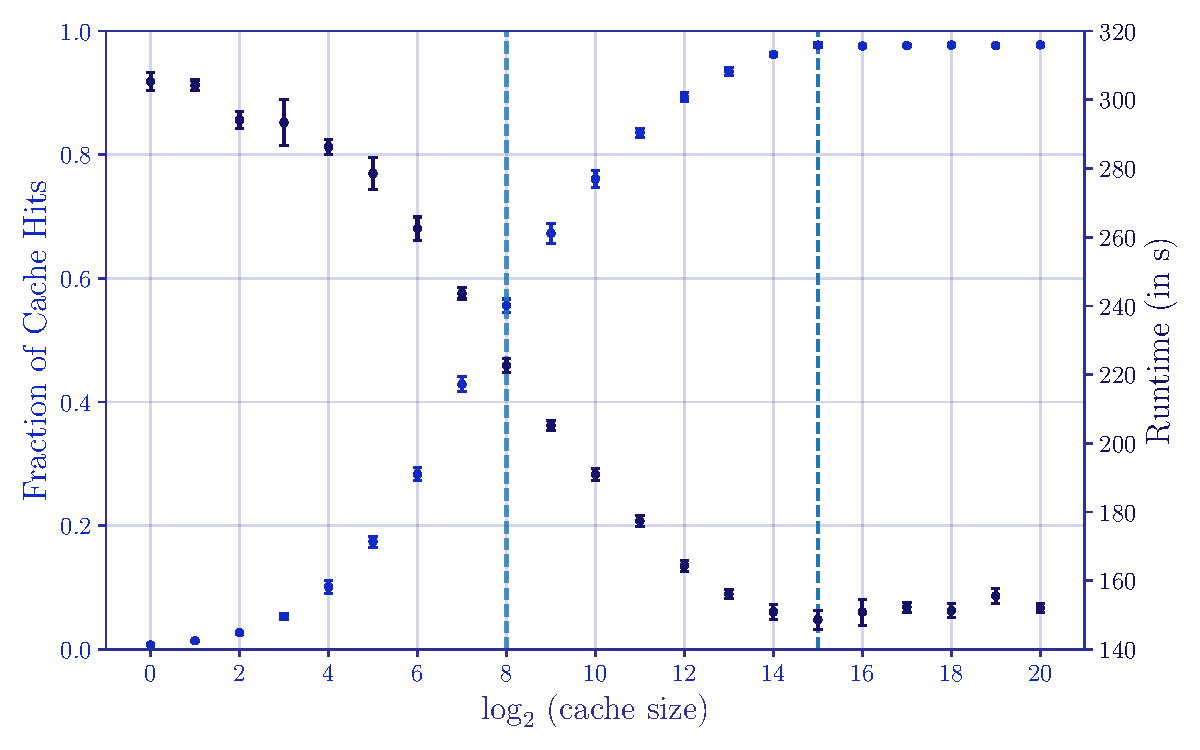
\includegraphics[width=0.8\linewidth]{graphics/chapter7/cacheSizeEffect.pdf}
    \vspace{0.5cm}
    \caption{Effect of the cache size on the cache hit rate (blue) and the runtime of the simulation (navy). The chosen cache sizes for further experiments, $2^8 = 256$ and $2^{15} = 32768$ are denoted by the vertical dashed line.}
    \label{fig:cacheSizeEffects}
\end{figure}

\subsection{Cache utilization and hit rates over time}

With the cache size fixed at $2^8$ and $2^{15}$ reaction instances, we analysed how cache utilization and hit rates evolve during the course of a simulation. The cache hit rate (blue) and the fraction of cache capacity utilized (navy) are shown in Figure~\ref{fig:cacheAccess}. Cache hit rate and utilization are two correlated measures of cache use: once the entire cache has been utilized, new instances would be added to the cache at the expense of existing instances and the hit rate would start to fall. Prior to that, the hit rate would be close to one, because any new instances can be added to the cache which has not yet reached its capacity.

In the closed system with cache size $2^8$ (Figure~\ref{fig:cacheNoFlow}), the cache is populated gradually over the first $1\times 10^5$ simulation steps. During this initial phase, the diversity of reactions is low and the system repeatedly applies a small set of reaction templates to the small set of molecular pairs. Consequently, the cache hit rate is high (nearly $100\%$). Once the cache is filled, new reaction instances are stored by evicting the least recently used cached entries. This eviction of reaction instances leads to a sharp decline in the hit rate, as expected, which stabilizes at approximately $56\pm 12\%$ after about $3\times 10^5$ steps.
This stabilization coincides with the system ending its generative phase: by this point, the total number of molecules, the maximum molecular length, and the number of unique molecular classes have all reached steady values, as seen in Figure~\ref{fig:distMolsNoFlow}. The reduced hit rate therefore reflects increased diversity in reaction requests during the earlier generative phase, followed by repeated sampling from a larger but fairly stable set of reactions.

In contrast, when inflows and outflows are enabled with a cache of size $2^8$ (Figure~\ref{fig:cacheFlow}), the cache fills much more rapidly, within the first $2\times 10^3$ steps. The cache hit rate drops sharply during the early stages of the simulation, indicating a higher initial diversity of reactions. This decline gradually decreases and stabilizes around $75\pm 8\%$ beyond the first $2\times 10^5$ steps.
The higher steady-state hit rate in the flow-enabled system reflects the lower molecular diversity maintained in the system under open conditions, as seen in Figure~\ref{fig:distMolsFlow}. Continuous inflow of methanal and outflow of larger molecules restricts the range of molecular classes present at any given time, reducing the number of distinct molecular pairs and reaction templates encountered.

\begin{figure}
    \centering
    \vspace{0.5cm}
    \begin{subfigure}{0.49\textwidth}
        \centering
        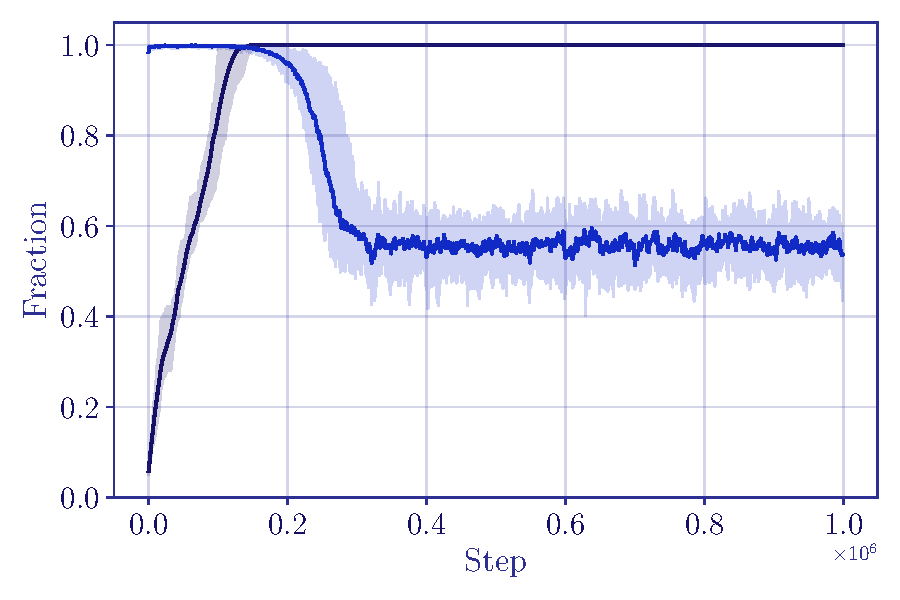
\includegraphics[width=\textwidth]{graphics/chapter7/cache_noFlow_256.pdf}
        \caption{Flows disabled and cache size $2^8$.}
        \label{fig:cacheNoFlow}
    \end{subfigure}% 
    \hfill
    \begin{subfigure}{0.49\textwidth}
        \centering
        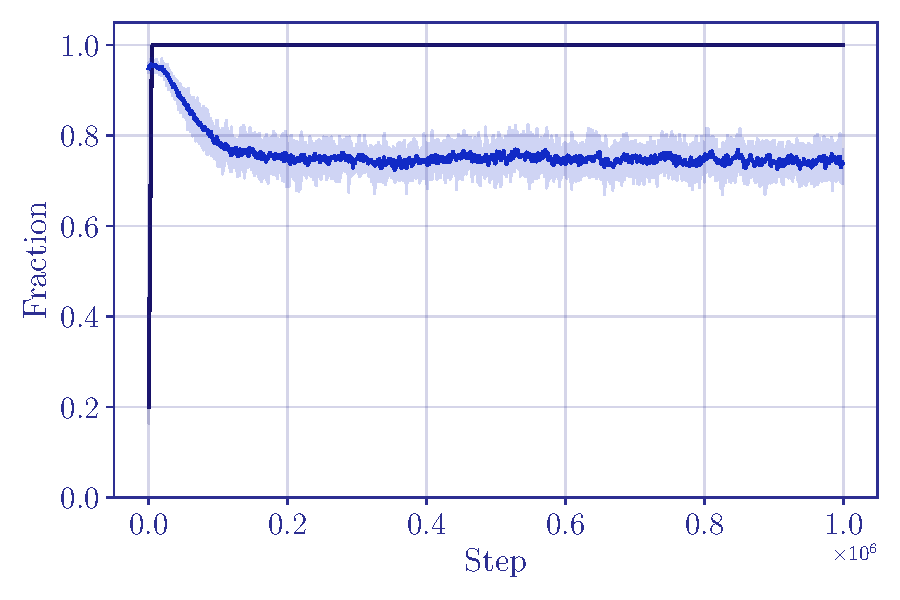
\includegraphics[width=\textwidth]{graphics/chapter7/cache_flow_256.pdf}
        \caption{Flows enabled and cache size $2^8$.}
        \label{fig:cacheFlow}
    \end{subfigure}\\
    \vspace{1.0cm}
    \begin{subfigure}{0.49\textwidth}
        \centering
        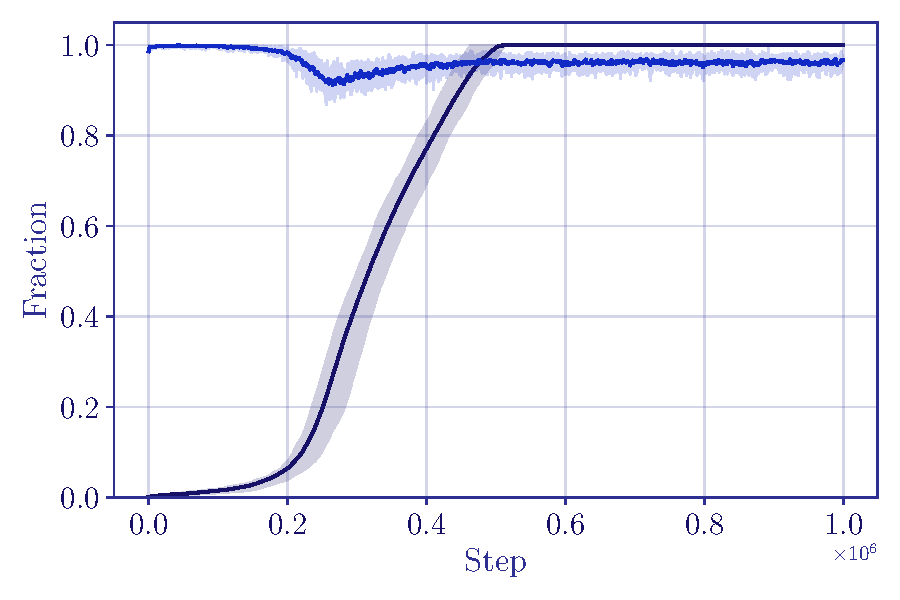
\includegraphics[width=\textwidth]{graphics/chapter7/cache_noFlow_32768.pdf}
        \caption{Flows disabled and cache size $2^{15}$.}
        \label{fig:bigCacheNoFlow}
    \end{subfigure}% 
    \hfill
    \begin{subfigure}{0.49\textwidth}
        \centering
        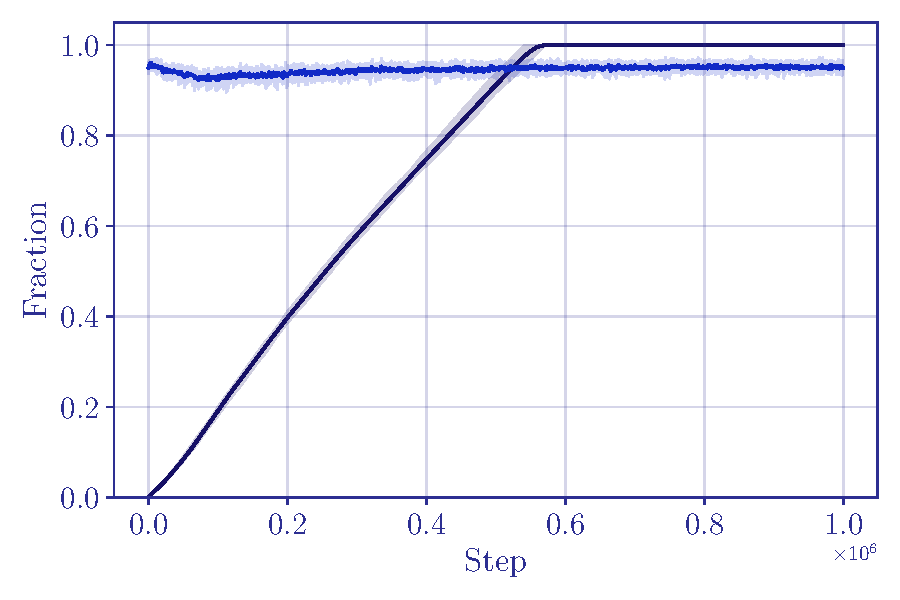
\includegraphics[width=\textwidth]{graphics/chapter7/cache_flow_32768.pdf}
        \caption{Flows enabled and cache size $2^{15}$.}
        \label{fig:bigCacheFlow}
    \end{subfigure}
    \vspace{0.5cm}
    \caption{Cache hit rate (blue) and fraction of utilization of the cache (navy) under the two different flow conditions and two different cache sizes.}
    \label{fig:cacheAccess}
\end{figure}

In the closed system with cache size $2^{15}$ (Figure~\ref{fig:bigCacheNoFlow}), the cache is populated over the first $5\times 10^5$ simulation steps. The cache is filled gradually in the initial phase consisting of the first $2\times 10^5$ steps, after which the cache utilization picks up pace. There is a slight dip in the cache hit rate at the beginning of this phase, where new reaction instances are explored by the system, which was not found in the cache. These are added to the cache (whose capacity is not reached yet) raising its utilization rate. The cache hit rate remains consistently high ($\sim 96\pm 3\%$) during the entire simulation, indicating that the cache at all times have capacity for holding the active set of reactions.

When flows are allowed along with using a cache size $2^{15}$ (Figure~\ref{fig:bigCacheFlow}), the cache is filled over the first $5\times 10^5$ simulation steps, with the rate being roughly similar over the entire phase. The cache hit rate is maintained at roughly $\sim 95\pm 3 \%$ over the entire simulation.

\subsection{Impact on runtime}

The primary motivation for introducing caching is to reduce the computational overhead associated with repeatedly enumerating reaction instances, particularly the costly subgraph isomorphism checks required to match reaction templates. Even though the underlying graph transformation engine MØD~\cite{mod_graphTransformation} is highly optimized, caching at the simulation level still yields measurable performance improvements. Caching does not alter the observables of the system (such as the distribution of the number of carbons in the molecules, the innovation rate for molecules or the relative abundances of different molecular classes or the trajectory of the simulation) and has no impact on the outcome of the stochastic exploration.

Table~\ref{tab:runtime} summarizes the average runtimes over 100 simulation trials, without and with caching (with different cache sizes). When flows are disabled and a cache of size $2^8$ is used, caching reduces the runtime by approximately $91$ seconds ($\sim 27\%$). With the same cache size, when flows are enabled, the reduction is approximately $59$ seconds ($\sim 16\%$).
The decrease in the runtime with cache size $2^{15}$ and without flows is approximately $187$ seconds ($\sim 56\%$), while with flows enabled, the reduction is approximately $160$ seconds ($\sim 42\%$).
Despite the higher cache hit rate observed in the flow-enabled system, the relative speedup is smaller. This is because cache hits only accelerate steps in which a chemical reaction is to be executed. Inflow and outflow steps—which constitute a substantial fraction of simulation steps when flows are enabled—do not benefit from caching. Since the cache hit rate is computed only over reaction steps, the overall fraction of accelerated steps is lower, leading to a smaller net reduction in runtime.

\begin{table}
	\centering
	\begin{footnotesize}
	\begin{tabular}{@{}lcc@{}}
	\toprule
	& Without flows & With inflows and outflows \\
	\midrule
	Caching disabled & $335\pm 7$ & $377\pm 7$  \\
	Cache size $2^8$ & $244\pm 2$ & $318\pm 5$  \\
	Cache size $2^{15}$ & $148\pm 3$ & $217\pm 2$ \\
	\bottomrule\\
	\end{tabular}
	\end{footnotesize}
	\caption{Average runtime of the $100$ trials of the simulation, in seconds, without and with caching (for two different cache sizes). The results when flows are enabled are listed in the right column.}
	\label{tab:runtime}
\end{table}

\begin{figure}
    \centering
    \vspace{0.5cm}
    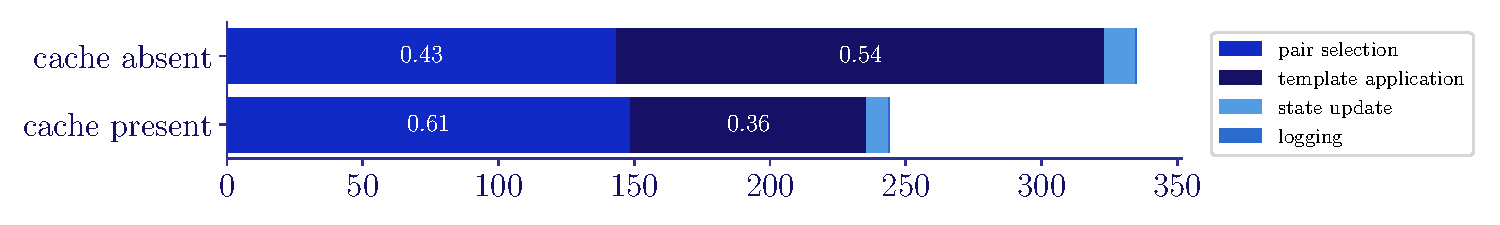
\includegraphics[width=0.9\linewidth]{graphics/chapter7/cache_fracTimes.pdf}
    \vspace{0.5cm}
    \caption{Breakdown of the total runtime of an average of $10$ trials of the simulation into what is spent on collision pair and reaction template selection (blue), template application or cache lookup on cache hit (navy), state update (cyan), and logging (aqua), when caching is disabled (top) and enabled (bottom). The labels (white) give the fraction of the total simulation time used for those components.}
    \label{fig:fracCacheTimes}
\end{figure}

Figure~\ref{fig:fracCacheTimes} gives the cost breakdown for the various components in the simulation, without and with a cache of size $2^{8}$. As described in Algorithm~\ref{generate_network}, choosing a transition out of the current state is divided into choosing a collision and a reaction template and then applying the chosen reaction template to the chosen molecules. Once the transition out of the current state is chosen, the state is updated and logged (if required). Without caching, the application of the reaction template on the molecular pair took more than half of the runtime. Using a cache to look up the results on a cache hit reduced template application time by a factor of two, leaving it at roughly one-third of the (now reduced) total simulation time.

With caching, we observe from Figure~\ref{fig:fracCacheTimes} that the fraction of runtime required to choose a pair of molecules from the state dictionary now is the largest part of the total runtime. This indicates that a next step in future work towards improving the proposed method might possibly be to try to optimize the choosing of the colliding pair of molecules, e.g.\ by improving on the data structures storing the state of the system.

\subsection{Cache as a partial record of network}

At the end of a simulation, the cache contains the most recently used reaction instances, effectively storing a subnetwork of the explored reaction network.
More precisely, as described in Section~\ref{cacheScheme}, each element of the cache stores a list of all reaction instances possible to generate by applying one template $r$ to one molecular pair $(m_1, m_2)$. It is the union of those lists that we consider the subnetwork represented by the cache.
Thus, while the stochastic simulation itself does not require explicit construction of the full reaction network, the cache provides a controllable, interpretable and lightweight representation of a portion of that network.

\begin{figure}[t]
    \centering
    \vspace{0.5cm}
    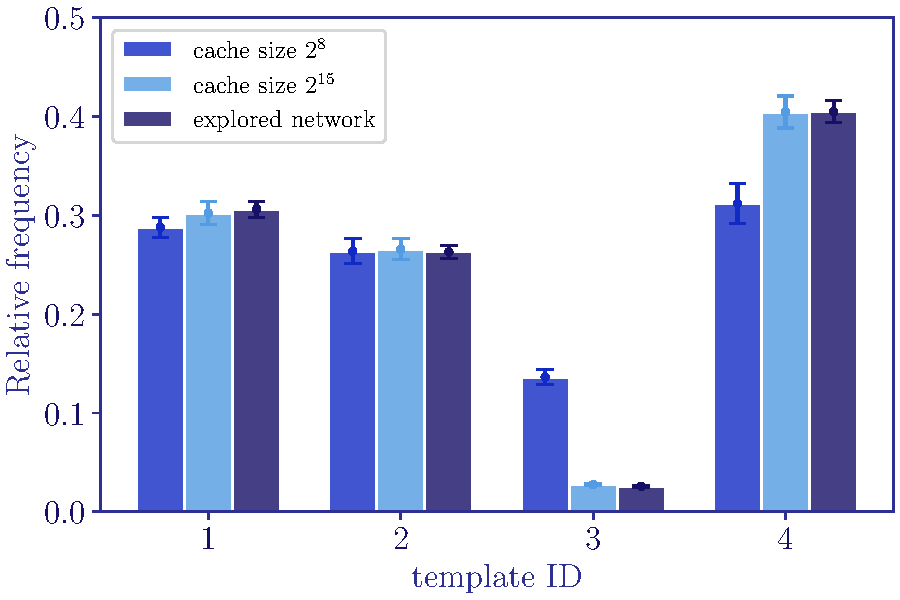
\includegraphics[width=0.75\textwidth]{graphics/chapter7/templateFreq.pdf}
    \vspace{0.5cm}
    \caption{Comparison of the relative distribution of the four reaction templates among the successful applications of a reaction template~$r$ on a molecular pair $(m_1,m_2)$. Successful means that the left-hand side of $r$ has one or more matches as a subgraph of $m_1 \cup m_2$. The blue bars show this for the contents of a cache of size~$2^8$ at the end of the simulation, the cyan bars show the same for a cache of size~$2^{15}$, and the navy bars show the distribution across all steps of the entire simulation. The error bars represent the standard deviation in the frequency over the $10$ trials conducted.}
    \label{fig:frequencyTemplate}
\end{figure}

By modifying the cache size or replacement policy, different regions of the explored network can be preferentially retained without altering the stochastic trajectory of the simulation. In the extreme case of a sufficiently large cache, all reaction instances encountered during the simulation would be retained, allowing reconstruction of the complete reaction network explored by the stochastic process. Therefore, the cache can be considered as a \emph{proxy} of the reaction network explored by the simulation. In this manner, the cache has a practical utility and a conceptual contribution to the analysis of the results of the simulation besides speeding it up. It might allow the possibility of analysing properties of the network without storing the entire enumerated reaction network.

To investigate to what extent the cached portion is representative of the entire explored network, we for caches of two sizes ($2^8$ and $2^{15}$) compared the coverage of reactions and molecules in their final state with that of the entire simulation.

Figure~\ref{fig:frequencyTemplate} shows the relative distribution of the four reaction templates among the successful applications of a reaction template~$r$ on a molecular pair $(m_1,m_2)$. Successful means that the left-hand side of $r$ has one or more matches as a subgraph of $m_1 \cup m_2$. The blue bars show this distribution for the keys stored in a cache of size~$2^8$ at the end of a simulation of $10^6$ steps (the keys of the cache have type $(r, m_1,m_2)$ and successful is equivalent to the list of the cache element being non-empty). The cyan bars show the same distribution for a cache of size~$2^{15}$. The navy bars show the same distribution for all steps of the entire simulation (but only counting the first successful application for each $(r, m_1,m_2)$ triple, not repetitions, to be consistent with the counting of the cache contents).
The error bars depict the standard deviation over $10$ trials of the simulation.
The relative ordering of the frequencies of the reaction templates (which result in reaction instances) remains the same in all three cases, with cache of size $2^8$, $2^{15}$ and the explored network, namely template $4$ is the most frequent, followed by $1$, $2$ and $3$. The absolute counts of the number of times the particular template appears in the cache with instantiated reaction differ slightly.
Reactions generated using template $2$ are overrepresented in the cache of size $2^8$ at the expense of reactions effected using template $3$. 
Using a cache of size $2^{15}$, the frequencies of the templates closely follow the frequencies of the templates instantiated in the entire explored network.

\begin{table}
	\centering
	\begin{footnotesize}
	\begin{tabular}{rrrr}
	\toprule
	{Number of carbon atoms} & {Cache size $2^8$} & {Cache size $2^{15}$} & {Explored network} \\
	\midrule
	1 & 1 & 1 & 1 \\
	2 & 2 & 2 & 2 \\
	3 & 3 & 3 & 3 \\
	4 & 5 & 5 & 5 \\
	5 & 9 & 9 & 9 \\
	6 & 17 & 17 & 17 \\
	7 & 30 & 34 & 34 \\
	> 7 & 48 & 426 & 431 \\
	\bottomrule\\
    \end{tabular}
    \end{footnotesize}
    \caption{A comparison of the number of classes of molecules with different number of carbon atoms in the two caches with different sizes.}
    \label{fig:molSizes}
\end{table}

Table~\ref{fig:molSizes} lists the number of molecular classes with increasing number of carbon atoms in the cached subnetwork, when cache size is $2^8$ and $2^{15}$, and the entire explored network, respectively. 
All the molecular classes with up to $6$ carbon atoms from the explored reaction network were present in both the caches. The molecular classes which are rarer and have more carbon atoms are the ones not present in the cache with size $2^8$: the cache contains only $48$ molecules with more than $7$ carbon atoms while there were $431$ such molecules in the entire explored network. The cache of size $2^{15}$ could capture $426$ of these $431$ molecules. Among the $115$ molecular classes in the cache with size $2^8$, $97\pm1$ of the $100$ most abundant molecular classes in the entire network were present. Out of the $100$ most frequently queried molecular pair-reaction template combinations during the simulation, $94\pm2$ were present in the cached subnetwork (with minor variations over trial runs). Thus, it was the rare molecular pair-reaction template queries that were absent in the cache, which is what would be expected from an efficient cache aiming to maximize the hit rate during the simulation.  
